\documentclass{beamer}
\usetheme{Madrid}
\usepackage{amssymb}
\usepackage{amsmath}
\usepackage{graphicx}

\makeatletter

\setbeamertemplate{footline}
{
  \leavevmode%
  \hbox{%
  \begin{beamercolorbox}[wd=.5\paperwidth,ht=2.25ex,dp=1ex,center]{author in head/foot}%
    \usebeamerfont{author in head/foot}\insertshortauthor
  \end{beamercolorbox}%
  \begin{beamercolorbox}[wd=.2\paperwidth,ht=2.25ex,dp=1ex,center]{title in head/foot}%
    \usebeamerfont{title in head/foot}\insertshorttitle
  \end{beamercolorbox}%
  \begin{beamercolorbox}[wd=.3\paperwidth,ht=2.25ex,dp=1ex,right]{date in head/foot}%
    \usebeamerfont{date in head/foot}\insertshortdate{}\hspace*{2em}
    \insertframenumber{} / \inserttotalframenumber\hspace*{2ex}
  \end{beamercolorbox}}%
  \vskip0pt%
}

\makeatother

\beamertemplatenavigationsymbolsempty

\title[UndeepVO]{UnDeepVO: Monocular Visual Odometry through Unsupervised Deep Learning}
\author{
    Bola\~nos T.\\
    \and
    Kilkkilä M.\\
    \and
    Kurki L.\\
    \and
    Rehn A.\\
    \and
    Zaka A.\\
    \and
    Zhao Z.
}
\date{\today}

\begin{document}

\begin{frame}
    \titlepage
\end{frame}

\begin{frame}
    \frametitle{Outline}
    \tableofcontents
\end{frame}

\section{Introduction}
\section{System Overview}
\section{Objective Losses}
\section{Experimental Evaluation}
\section{Conclusion}
\section{Contributors}

\begin{frame}
    \frametitle{Introduction}
    \framesubtitle{UnDeepVO}
    \begin{itemize}
        \item A monocular visual odometry system
        \item Paper by Ruihao Li, Seng Wang, Zhiqiang Long and Dongbing Gu
    \end{itemize}
\end{frame}

\begin{frame}
    \frametitle{Introduction}
    \framesubtitle{Visual odometry}
    \begin{itemize}
        \item Goal
        \begin{itemize}
            \item Robot localization using only visual information
        \end{itemize}
    \end{itemize}
    \begin{figure}
        
\includegraphics[scale=0.8]{images/road1.png}
        
\includegraphics[scale=0.8]{images/road2.png}
        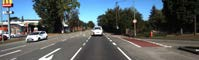
\includegraphics[scale=0.8]{images/road3.png}
        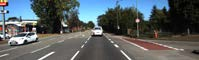
\includegraphics[scale=0.8]{images/road4.png}
    \end{figure}
\end{frame}

\begin{frame}
    \frametitle{Introduction}
    \framesubtitle{Visual odometry}
    \begin{itemize}
        \item Goal
        \begin{itemize}
            \item Use consecutive monocular images to construct a path of robot movement
        \end{itemize}
    \end{itemize}
    \begin{figure}
        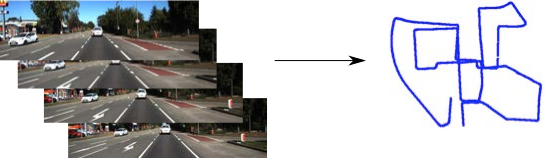
\includegraphics[scale=0.8]{images/vo-objective.png}
    \end{figure}
\end{frame}

\begin{frame}
    \frametitle{Introduction}
    \framesubtitle{UnDeepVO}
    \begin{itemize}
        \item Based on deep learning
        \item Unsupervised
        \begin{itemize}
            \item No need for labeled training data
        \end{itemize}
        \item Pose estimation
        \item Depth estimation
    \end{itemize}
\end{frame}

\begin{frame}
    \frametitle{System Overview}
    \framesubtitle{Architecture}
    \begin{itemize}
        \item Maybe that figure on the paper ...
    \end{itemize}
\end{frame}

\begin{frame}
    \frametitle{System Overview}
    \framesubtitle{Training Scheme}
    \begin{itemize}
        \item ...
    \end{itemize}
\end{frame}

\begin{frame}
    \frametitle{Objective Losses}
    \framesubtitle{Spatial Losses}
    The spatial losses are based on the fact that, given the structure of stereo cameras, for a pixel $p_l(u_l, v_l)$ on the left image and $p_r(u_r, v_r)$ on the left image:

    \[ u_l = u_r \hspace{1em} \text{and} \hspace{1em} v_l = v_r + D_p \] 
    \begin{itemize}
        \item Photometric Consistency Loss (Image reconstruction)
        \[ L_{pho} = \lambda_s L^{SSIM} (I, I') + (1 - \lambda_s)L^{l_1}(I, I') \]

        \item Disparity Consistency Loss (Depth)
        \[ L_{dis} = L^{l_1}(D_{dis}, D_{dis}') \]

        \item Pose Consistency Loss (Camera orientation)
        \[ L_{pos} = \lambda_pL^{l_1}(t_l, t_r) + \lambda_oL^{l_1}(R_l, R_r) \]
    \end{itemize}
\end{frame}

\begin{frame}
    \frametitle{Objective Losses}
    \framesubtitle{Temporal Losses}
    This is based on the reconstruction of pixels on time $k$ and $(k + 1)$ as
    \[p_{k + 1} = K T_{k, k+1} D_{dep} K^{-1} p_k \]
    \begin{itemize}
        \item Photometric Consistency Loss (Image reconstruction)
        \[ L_{pho} = \lambda_s L^{SSIM} (I, I') + (1 - \lambda_s)L^{l_1}(I, I') \]

        \item 3D Geometric Registration Loss (Adding depth with $P(x, y, z)$)
        \[ L_{geo} = L^{l_1} (P, P') \]

    \end{itemize}
\end{frame}

\begin{frame}
    \frametitle{Evaluation}
    \framesubtitle{Trajectory}
	       \begin{columns}
	       	\begin{column}{0.48\textwidth}
	       		\begin{itemize}
	       			\item KITTI Odometry Dataset 
	       			\item Comparison between UnDeepVO, SfMLearner VISO2-M and ORB-SLAM-M
	       			\item UnDeepVO qualitatively closest to the ground truth for all sequences
	       		\end{itemize}
	       	\end{column}
	       	\begin{column}{0.48\textwidth}
	       	\vspace{-.5cm}
	    	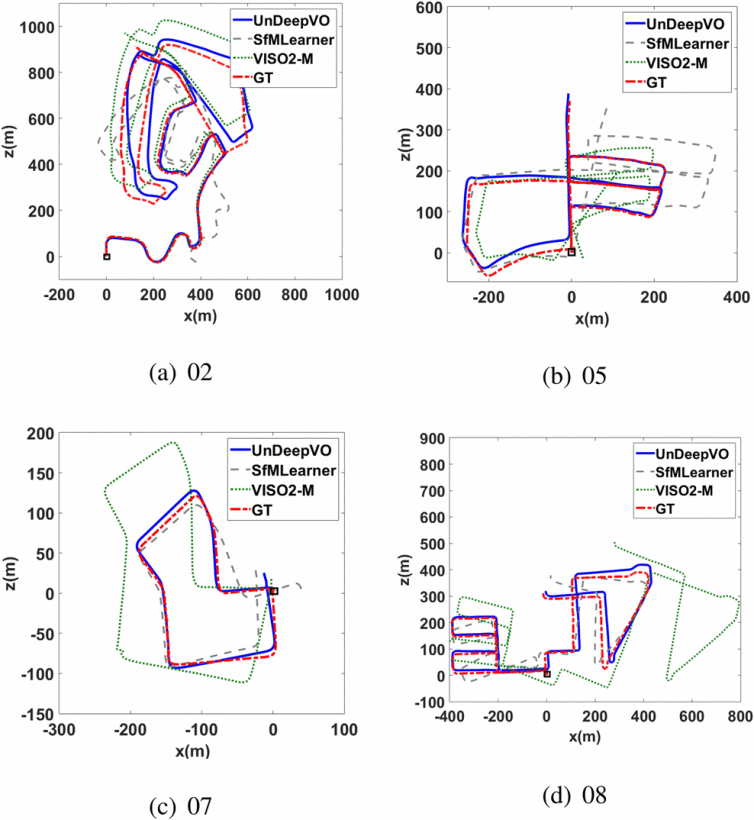
\includegraphics[width=\linewidth]{images/trajectory-eval.png}
	       	\end{column}
	       \end{columns} 

\end{frame}

\begin{frame}
    \frametitle{Evaluation}
    \framesubtitle{Depth}
	       \begin{columns}
	       	\begin{column}{0.45\textwidth}
	       		\begin{itemize}
	       			\item UnDeepVO also produces a scaled depth map 
	       			\item Depth of objects estimated accurately
	       			\item Model outperforms some competitors but not all
	       			\begin{itemize}
	       				\item Only part of KITTI dataset used
	       				\item Lower image resolution
	       				\item Temporal image sequence loss might have introduced noise
	       			\end{itemize}
	       				       			
	       		\end{itemize}
	       	\end{column}
	       	\begin{column}{0.53\textwidth}
	       		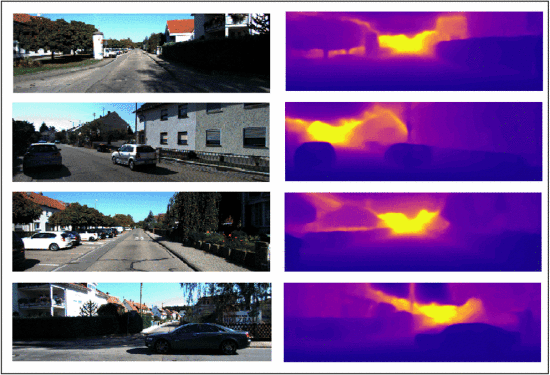
\includegraphics[width=\linewidth]{images/depth_estimation.png}
	       	\end{column}
	       \end{columns} \end{frame}

\begin{frame}
    \frametitle{Conclusions}
    \begin{itemize}
        \item Performs inference on monocular images
        \item Pose and dense estimations for recovering the trajectory
            \begin{itemize}
                \item One CNN for depth estimation
                \item Another CNN for pose estimation
            \end{itemize}
        \item Outperforms previous methods in almost all cases
        \item First unsupervised Visual Odometry model
        \begin{itemize}
            \item Trained with unlabeled stereo images
            \item Uses stereo image pairs to recover the scale
            \item Scale can not be recovered from monocular images
        \end{itemize}
        \item Plans to extend to a SLAM system
    \end{itemize}
\end{frame}

\begin{frame}
    \frametitle{Contributors}
    \begin{itemize}
        \item Bola\~nos Tlahui
            \begin{itemize}
                \item Objective Losses
            \end{itemize}
        \item Kilkkilä Miikka
            \begin{itemize}
                \item ...
            \end{itemize}
        \item Kurki Lauri
            \begin{itemize}
                \item ...
            \end{itemize}
        \item Rehn Aki
            \begin{itemize}
                \item Slide organization, introduction, conclusions
            \end{itemize}
        \item Zaka Ayesha
            \begin{itemize}
                \item UnDeep VO Key Contributions
            \end{itemize}
        \item Zhao Zhao
            \begin{itemize}
                \item System Overview
            \end{itemize}
    \end{itemize}
\end{frame}


\end{document}
